\documentclass[dvipdfmx,autodetect-engine,titlepage]{jsarticle}
\usepackage[dvipdfm]{graphicx}
\usepackage{ascmac}
\usepackage{fancybox}
\usepackage{listings}
\usepackage{plistings}
\usepackage{itembkbx}
\usepackage{amsmath}
\usepackage{svg}
\usepackage{url}
\usepackage{graphics}
\usepackage{listings,jvlisting}
\usepackage{scalefnt}

\textheight=23cm
\renewcommand{\figurename}{図}
\renewcommand{\tablename}{表}
\newenvironment{code}
{\vspace{0.5zw}\VerbatimEnvironment  
\begin{screen} 
\baselineskip=1.0\normalbaselineskip
 \begin{Verbatim}}
{\end{Verbatim}
\baselineskip=\normalbaselineskip
 \end{screen}\vspace{0.5zw}} 

 \lstset{
    basicstyle={\ttfamily},
    identifierstyle={\small},
    commentstyle={\smallitshape},
    keywordstyle={\small\bfseries},
    ndkeywordstyle={\small},
    stringstyle={\small\ttfamily},
    frame={tb},
    breaklines=true,
    columns=[l]{fullflexible},
    numbers=left,
    xrightmargin=0zw,
    xleftmargin=3zw,
    numberstyle={\scriptsize},
    stepnumber=1,
    numbersep=1zw,
    lineskip=-0.5ex
    }

\title{情報理工学部 SNコース 2回\\
セキュリティ・ネットワーク学実験2\\
課題5-3レポート}
\author{2600200443-6\\Yamashita Kyohei\\山下 恭平}
\date{December 17 2021}

\begin{document}

\maketitle

\section{概要}
接続許可リストにあるクライアントのみに対し,クライアントから送られて
きた文字列を変換し,クライアントへ返送する TCP サーバプログラムを作成する。


\section{外部仕様}

\subsection{サーバ側}
サーバは起動と同時に図1の状態になり、クライアントからの接続を待っている状態となる。
許可したIPアドレスから接続が行われた時「conected :接続先IPアドレス」と表示され、
許可されていないIPアドレスからの接続が行われた場合は、そのIPアドレスを表示し、
「許可されていないIPアドレスからのアクセス」と表示されるようになっている。その
様子を図2,3に示す。
\begin{figure}[h]
    \centering
    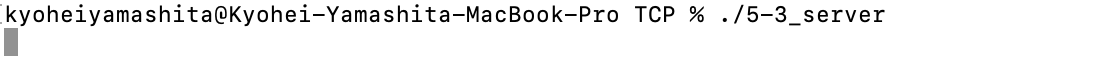
\includegraphics[scale=1]{pic11.png}
    \caption{接続待ち状態}
  \end{figure}

\begin{figure}[h]
    \centering
    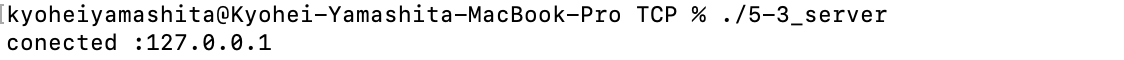
\includegraphics[scale=1]{pic7.png}
    \caption{許可した相手からの接続}
  \end{figure}

  \begin{figure}[h]
    \centering
    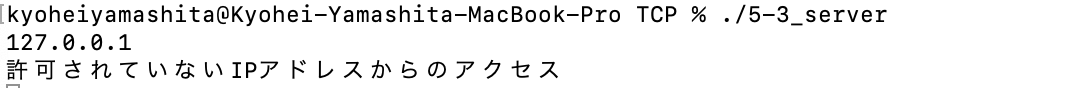
\includegraphics[scale=1]{pic9.png}
    \caption{許可していない相手からの接続}
  \end{figure}


\subsection{クライアント側}
クライアント側は図4のように、起動時、第二引数にホスト名、第三引数にポート番号を
指定することで接続先を任意に指定することができる。自身のIPアドレスがサーバへの接続
を許可されていた場合図5のように接続先のIPアドレスを表示し、送信するメッセージをキーボード
から受け付けるようになっている。もし、自身のIPアドレスがサーバの許可を得ていない場合
、図6のように接続が拒否された趣旨のメッセージを表示するようになっている。

\begin{figure}[h]
    \centering
    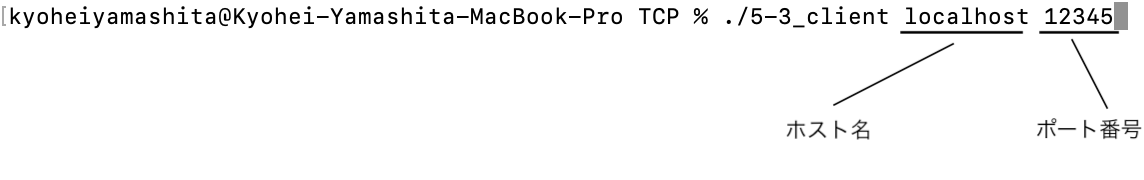
\includegraphics[scale=0.8]{pic5.png}
    \caption{接続方法}
  \end{figure}

  \begin{figure}[h]
    \centering
    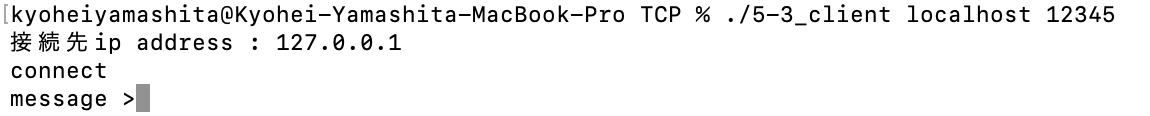
\includegraphics[scale=0.85]{pic6.png}
    \caption{接続した時}
  \end{figure}

  \begin{figure}[h]
    \centering
    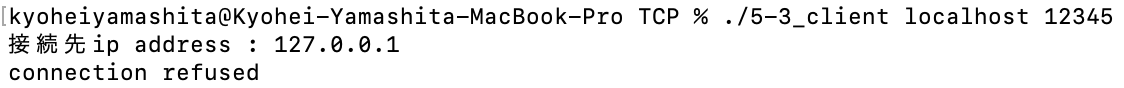
\includegraphics[scale=0.85]{pic8.png}
    \caption{接続が許可されていない場合}
  \end{figure}


\section{内部仕様}
\subsection{サーバ側}
サーバは「acceptlist.txt」に書き込まれているIPアドレスをfgetsで一行ずつ読み込み、
接続先のIPアドレスと比較していき、もし一致するものがあれば、接続先のIPアドレスを表示、
「threadfunc」を呼び出し、クライアント側の入力を待機、送られてきた文字列を大文字に変換し、
送信し返すようになっている。もし、一致するIPアドレスが存在しなかった場合、接続先のIPアドレスと
「許可されていないIPアドレスからのアクセス」を表示し、「refusefunc」を呼び出し、
bufに「refuzed」と書き込み、それを送信するようにしている。以下は、「acceptlist.txt」の例である。

\begin{lstlisting}[caption=acceptlist,label=txt]
  192.168.11.12
  192.168.11.14
  127.0.0.1    
  
\end{lstlisting}

\subsection{クライアント側}
クライアント側はコマンドライン引数の第二引数にホスト名、第三引数にポート番号が格納
されており、その情報をもとにソケットを生成し、サーバに接続する。サーバに接続後、サーバ
からのパケットを待機する。もし初めに送信されてきたデータに「refuzed」と書き込まれて
いた場合、自身のIPアドレスはサーバへの接続は許可されていないので「このIPアドレスから
の接続は許可されていません」と表示し、通信を終了する。「refuzed」と書き込まれていない
場合、送信するメッセージをキーボードから受け付け、それをサーバへ送信し、変換された
文字を受信、その文字を表示し通信を終了する。


\section{実行例}
今回の実験では実験室に設置されているコンピュータをクライアント、自身のコンピュ
ータをサーバとし、実験を行った。まず初めに自席に設置されているコンピュータの
IPアドレスは「172.27.74.63」であったので、このIPアドレスを「acceptlist.txt」
に書き込み、サーバを建て、クライアントから接続を行なったものが実行例1である。以下は
その実際の様子を示したものである。

\begin{figure}[h]
    \centering
    \begin{minipage}[b]{0.45\linewidth}
    \begin{center}
      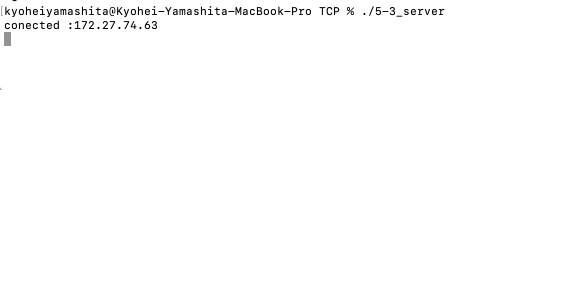
\includegraphics[keepaspectratio,scale=0.45]{pic3.png}
      \end{center}
      \caption{実行例1 サーバ}
    \end{minipage}
    \begin{minipage}[b]{0.45\linewidth}
    \begin{center}
      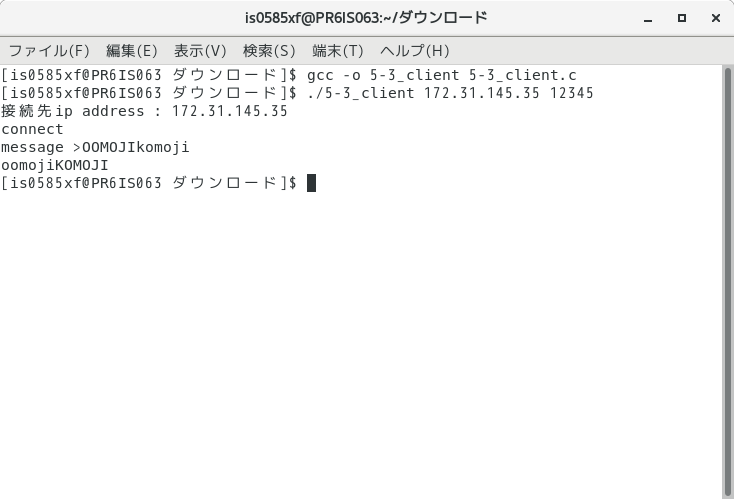
\includegraphics[keepaspectratio,scale=0.35]{pic1.png}
      \end{center}
      \caption{実行例1 クライアント}
    \end{minipage}
  \end{figure}

  実行例2では、逆に「acceptlist.txt」から自席のコンピュータのIPアドレスを
  削除し、サーバを建て実行したものである。実行結果は以下の図のとおりであり、
  仕様通り、サーバ側では接続先のIPアドレスがサーバに表示され、許可されていない
  との趣旨が表示され、クライアント側では接続が拒否されたことを示す内容を画面に
  表示している。


  \begin{figure}[h]
    \centering
    \begin{minipage}[b]{0.45\linewidth}
    \begin{center}
      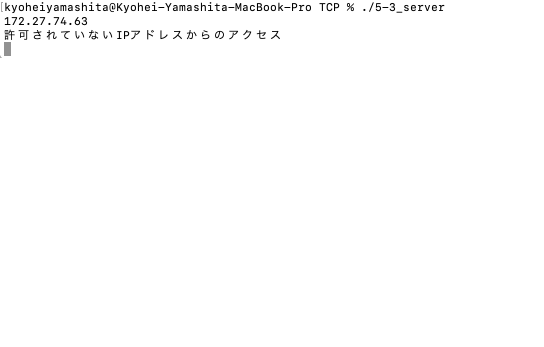
\includegraphics[keepaspectratio,scale=0.45]{pic4.png}
      \end{center}
      \caption{実行例2 サーバ}
    \end{minipage}
    \begin{minipage}[b]{0.45\linewidth}
    \begin{center}
      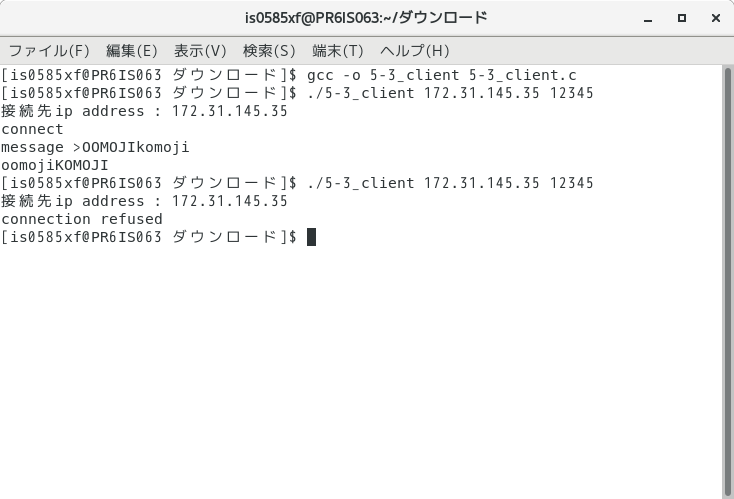
\includegraphics[keepaspectratio,scale=0.35]{pic2.png}
      \end{center}
      \caption{実行例2 クライアント}
    \end{minipage}
  \end{figure}

  実行例3は複数クライアントからの接続を行う実験である。「acceptlist.txt」
  には自身のコンピュータのIPアドレス「192.168.11.14」を書き込み、ローカル
  ホストである「127.0.0.1」は書き込まなかった。実行結果は、以下の図のとおり
  となり、マルチクライアント環境においても、IPアドレスによる判別ができていることが
  わかる。
  \begin{figure}[h]
    \centering
    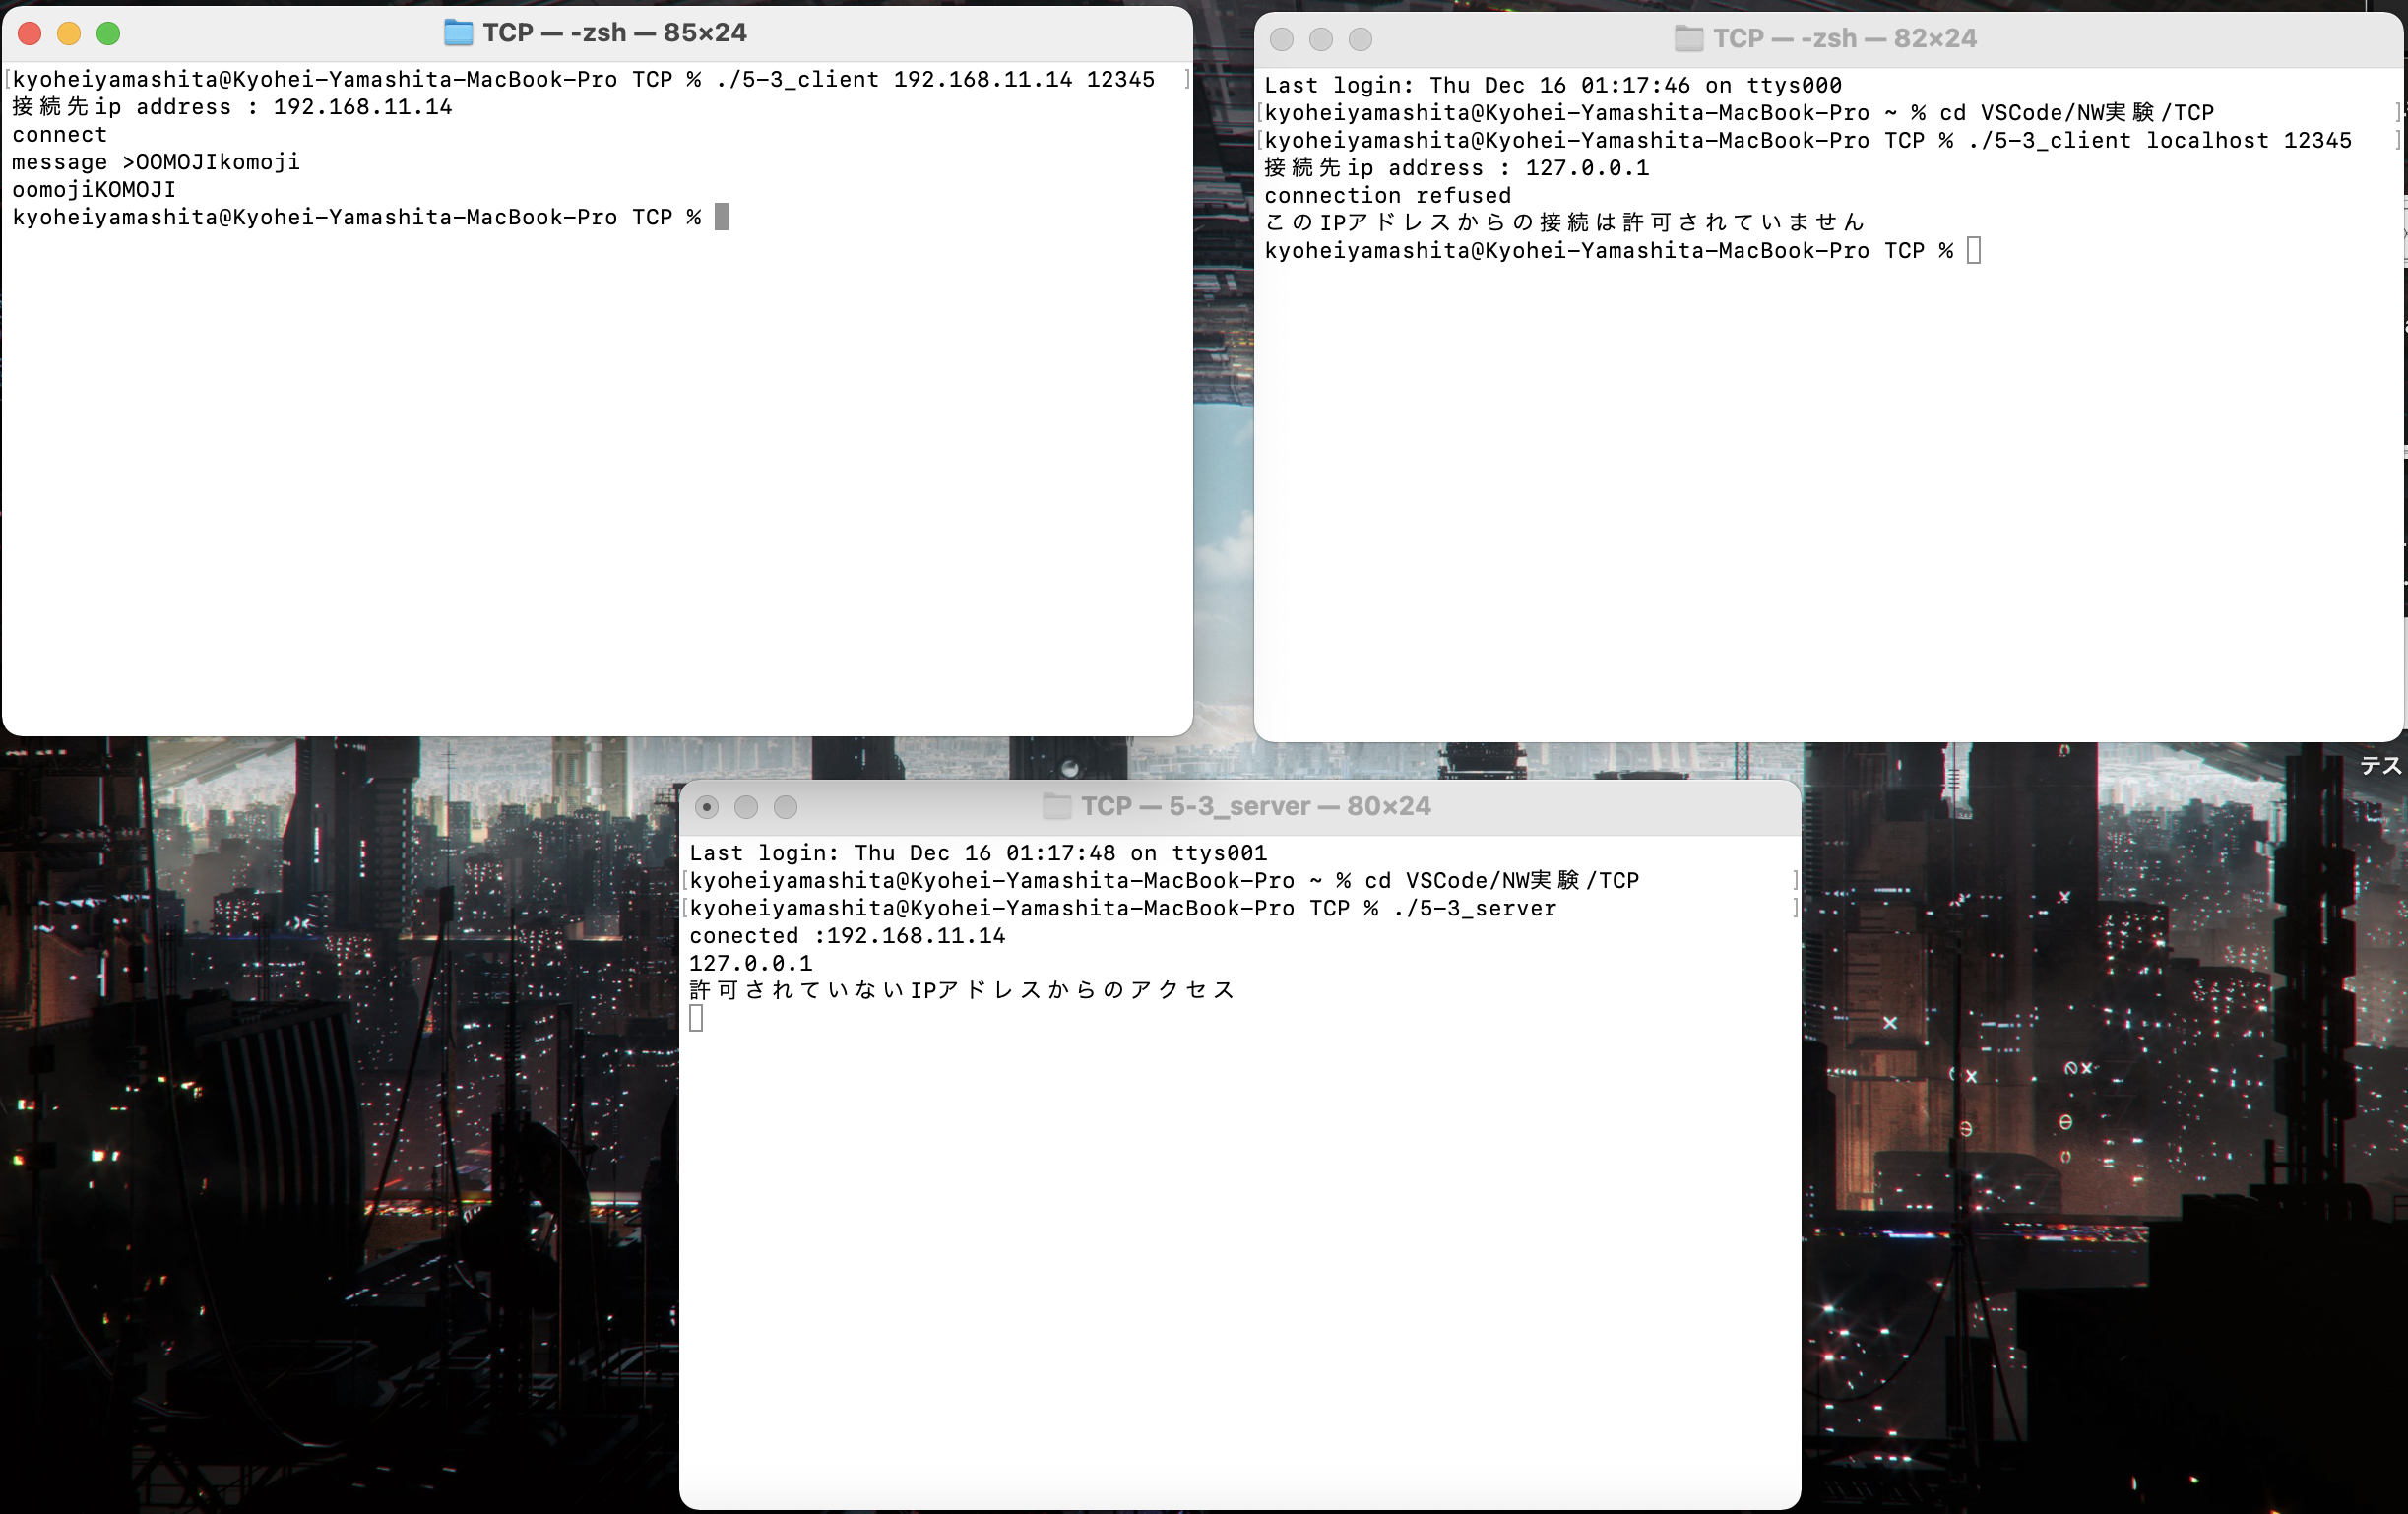
\includegraphics[scale=0.2]{pic10.png}
    \caption{実行例3 マルチキャスト}
  \end{figure}

\section{ソースコード}
\subsection{サーバ側}
\begin{lstlisting}[caption=server,label=server.c]
    #include <stdio.h>
    #include <unistd.h>
    #include <stdlib.h>
    #include <sys/types.h>
    #include <sys/socket.h>
    #include <netinet/in.h>
    #include <arpa/inet.h>
    #include <pthread.h>
    #include <errno.h>
    #include <string.h>
    
    struct clientdata
    {
        int sock;
        struct sockaddr_in saddr;
    };
    
    void *threadfunc(void *data)
    {
        int sock;
        struct clientdata *cdata = data;
        char buf[1024];
        int n, i, errocheck;
    
        if (data == NULL)
        {
            return (void *)-1;
        }
    
        /* (5)新規TCPコネクションのソケットを取得 */
        sock = cdata->sock;
    
        strcpy(buf, "connect");
    
        errocheck = write(sock, buf, sizeof(buf));
        if (errocheck < 0)
        {
            perror("write");
            goto err;
        }
    
        n = read(sock, buf, sizeof(buf));
        if (n < 0)
        {
            perror("read");
            goto err;
        }
    
        for (i = 0; buf[i] != '\0'; i++)
        {
            if ('a' <= buf[i] && buf[i] <= 'z')
            {
                buf[i] = buf[i] - ('a' - 'A');
            }
            else
            {
                buf[i] = buf[i] + ('a' - 'A');
            }
        }
    
        buf[i - 1] = '\0';
    
        n = write(sock, buf, n);
        if (n < 0)
        {
            perror("write");
            goto err;
        }
    
        /* 新規TCPセッションの終了 */
        if (close(sock) != 0)
        {
            perror("close");
            goto err;
        }
        /* 親スレッドでmallocされた領域を開放 */
        free(data);
    
        return NULL;
    
    err:
        free(data);
        return (void *)-1;
    }
    
    void *refusefunc(void *data)
    {
        int sock;
        struct clientdata *cdata = data;
        char buf[1024];
        int n, i;
    
        if (data == NULL)
        {
            return (void *)-1;
        }
    
        /* (5)新規TCPコネクションのソケットを取得 */
        sock = cdata->sock;
    
        strcpy(buf, "refused");
    
        n = write(sock, buf, sizeof(buf));
        if (n < 0)
        {
            perror("write");
            goto err;
        }
    
        /* 新規TCPセッションの終了 */
        if (close(sock) != 0)
        {
            perror("close");
            goto err;
        }
        /* 親スレッドでmallocされた領域を開放 */
        free(data);
    
        return NULL;
    
    err:
        free(data);
        return (void *)-1;
    }
    
    int main()
    {
        int sock0;
        struct sockaddr_in addr;
        socklen_t len;
        pthread_t th;
        struct clientdata *cdata;
    
        FILE *fp; // FILE型構造体
        char fname[] = "acceptlist.txt";
        char str[256];
    
        int refusecheck;
    
        /* (1) */
        /* ソケットの作成 */
        sock0 = socket(AF_INET, SOCK_STREAM, 0);
    
        /* ソケットの設定 */
        addr.sin_family = AF_INET;
        addr.sin_port = htons(12345);
        addr.sin_addr.s_addr = INADDR_ANY;
    
        bind(sock0, (struct sockaddr *)&addr, sizeof(addr));
    
        /* TCPクライアントからの接続要求を待てる状態にする */
        listen(sock0, 5);
        /* (1) 終わり */
    
        /* (2)新規TCPコネクションに関する情報をclientdata構造体に格納 */
        for (;;)
        {
            refusecheck = 0;
    
            cdata = malloc(sizeof(struct clientdata));
            if (cdata == NULL)
            {
                perror("malloc");
                return 1;
            }
    
            /* TCPクライアントからの接続要求を受け付ける */
            len = sizeof(cdata->saddr);
            cdata->sock = accept(sock0, (struct sockaddr *)&cdata->saddr, &len);
    
            fp = fopen(fname, "r"); // ファイルを開く。失敗するとNULLを返す。
            if (fp == NULL)
            {
                printf("%s file not open!\n", fname);
                return -1;
            }
    
            while (fgets(str, 256, fp) != NULL)
            {
                int l = 0;
    
                while (1)
                {
                    if (str[l] == '\n')
                    {
                        str[l] = '\0';
                        break;
                    }
    
                    l++;
                }
    
                if (strcmp(str, inet_ntoa(cdata->saddr.sin_addr)) == 0)
                {
                    printf("conected :%s\n", str);
    
                    refusecheck = 1;
    
                    /* (3)threadfunc()の処理を新スレッドとして実行 */
                    if (pthread_create(&th, NULL, threadfunc, cdata) != 0)
                    {
                        perror("pthread_create");
                        return 1;
                    }
    
                    /* (4)親スレッド側で子スレッドをdetach */
                    if (pthread_detach(th) != 0)
                    {
                        perror("pthread_detach");
                        return 1;
                    }
    
                    fclose(fp);
    
                    break;
                }
            }
    
            if (refusecheck == 0)
            {
                
                printf("%s\n",inet_ntoa(cdata->saddr.sin_addr));
    
                puts("許可されていないIPアドレスからのアクセス");
    
                if (pthread_create(&th, NULL, refusefunc, cdata) != 0)
                {
                    perror("pthread_create");
                    return 1;
                }
    
                /* (4)親スレッド側で子スレッドをdetach */
                if (pthread_detach(th) != 0)
                {
                    perror("pthread_detach");
                    return 1;
                }
            }
        }
    
        /* (8) */
        /* listen するsocketの終了 */
        if (close(sock0) != 0)
        {
            perror("close");
            return 1;
        }
    
        return 0;
    }
    
    
    
\end{lstlisting}

\subsection{クライアント側}
\begin{lstlisting}[caption=client,label=client.c]
#include <stdio.h>
#include <stdlib.h>
#include <string.h>
#include <unistd.h>
#include <sys/types.h>
#include <sys/socket.h>
#include <netinet/in.h>
#include <arpa/inet.h>
#include <errno.h>
#include <netdb.h>

int main(int argc, char *argv[])
{
    struct sockaddr_in server;
    struct addrinfo hints, *res;
    struct in_addr addr;
    int sock;
    char buf[1024];
    int n;
    int errocheck;
    int portnum;
    char ipadd[16];

    portnum = atoi(argv[2]);

    memset(&hints, 0, sizeof(hints));
    hints.ai_socktype = SOCK_STREAM;
    hints.ai_family = AF_INET;
    if ((errocheck = getaddrinfo(argv[1], NULL, &hints, &res)) != 0)
    {
        printf("error %d\n", errocheck);
        return 1;
    }

    addr.s_addr = ((struct sockaddr_in *)(res->ai_addr))->sin_addr.s_addr;
    inet_ntop(AF_INET, &addr, ipadd, sizeof(ipadd));
    printf("ip address : %s\n", ipadd);

    /* ソケットの作成 */
    sock = socket(AF_INET, SOCK_STREAM, 0);
    if (sock < 0)
    {
        perror("socket");
        printf("%d\n", errno);
        return 1;
    }

    /* 接続先指定用構造体の準備 */
    server.sin_family = AF_INET;
    server.sin_port = htons(portnum);

    /* 127.0.0.1はlocalhost */
    inet_pton(AF_INET, ipadd, &server.sin_addr.s_addr);

    /* サーバに接続 */
    errocheck = connect(sock, (struct sockaddr *)&server, sizeof(server));
    if (errocheck < 0)
    {
        perror("connect");
        printf("%d\n", errno);
        return 1;
    }

    read(sock, buf, sizeof(buf));

    if (strcmp(buf, "refused") == 0)
    {
        puts("connection refused");

        close(sock);

        freeaddrinfo(res);

        return 0;
    }
    else
    {
        printf("%s\n",buf);

        printf("message >");

        fgets(buf, 1024, stdin);

        write(sock, buf, sizeof(buf));

        read(sock, buf, sizeof(buf));

        printf("%s\n", buf);

        /* socketの終了 */
        close(sock);

        freeaddrinfo(res);

        return 0;
    }
}



\end{lstlisting}


\end{document}

